
\section{Coordenadas Ecuatoriales}\label{apendice:ecuatorial}

En este sistema, el ecuador celeste es la intersección del plano ecuatorial de la Tierra con la esfera celeste. Los polos celestes coinciden con los polos terrestres, además los círculos máximos que pasan por los polos celestes se denominan meridianos. La ascensión recta $\alpha$ es el ángulo en el plano ecuatorial que va desde el punto vernal hasta el meridiano del objeto. El punto vernal es el punto sobre la esfera celeste donde se intersectan el ecuador celeste y la eclíptica en el equinoccio vernal, este es el equinoccio de Otoño en el hemisferio sur. La declinación $\delta$ es el ángulo de elevación con respecto al plano ecuatorial.


Las coordenadas ecuatoriales de un objeto cambian lentamente año tras año debido a la precesión del eje de rotación de la Tierra, con un período de $\sim$25770 años con respecto a un eje perpendicular al plano de la elíptica. Debido a que las coordenadas ecuatoriales están fijas al ecuador terrestre y relativas al equinoccio vernal, el sistema de coordenadas se mueve conforme la Tierra precede. 

\section{Coordenadas Locales} \label{apendice:local}

El sistema de coordenadas locales, localiza los objetos de acuerdo a un sistema centrado en la posición del observador. El ecuador en este sistema está definido por la intersección del plano tangente a la superficie de la Tierra en la ubicación del observador y la esfera celeste. 


La localización de un objeto está dada por dos ángulos: el ángulo cenital $\theta$ que se mide desde un punto de la esfera celeste directamente arriba del observador, este punto es llamado  cenit. El segundo ángulo es el azimutal $\phi$ medido sobre el plano ecuatorial tomando como referencia algún punto, por ejemplo, el observatorio Pierre Auger define el cero hacia el Este y crece en dirección Norte, en sentido anti-horario. El ángulo cenital mide ángulos entre -90$^o$ y 90$^o$ aunque la parte negativa no es visible por el observador. El azimut recorre desde 0$^o$ hasta 360$^o$. Se debe tener en cuenta además que este sistema al estar fijo con el observador se mueve con la rotación de la Tierra.


\begin{figure}[H]
    \begin{small}
        \begin{center}
            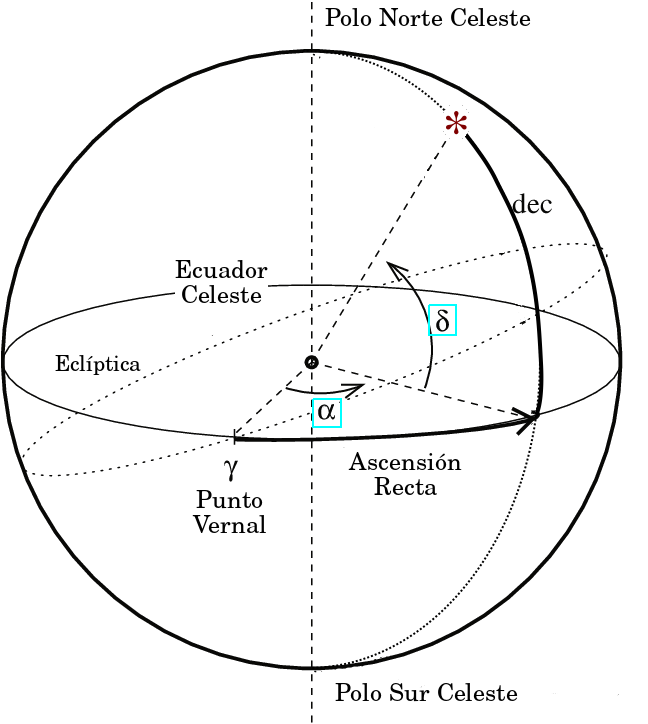
\includegraphics[width=0.6\textwidth]{EC.png}
        \end{center}
        \caption{Esquema de las coordenadas ecuatoriales de un punto cualquiera sobre la esfera celeste.}
        \label{fig:}
    \end{small}
\end{figure}

\begin{figure}[H]
    \begin{small}
        \begin{center}
            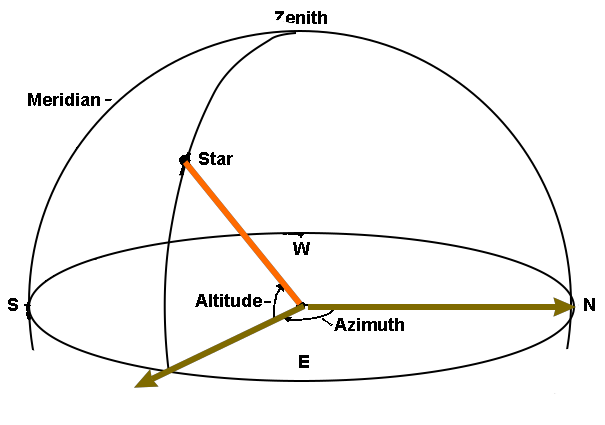
\includegraphics[width=0.75\textwidth]{LC.png}
        \end{center}
        \caption{Esquema de las coordenadas locales de un punto cualquiera sobre la esfera celeste.}
        \label{fig:}
    \end{small}
\end{figure}

